\section{Experimental Evaluation}
\label{sec:evaluation}

We evaluate the performance of CapsuleGANs at randomly generating images through a series of experiments as described below, in which we compare CapsuleGANs with convolutional GANs both qualitatively and quantitatively. We implement both the GAN models with the same architecture for their generators. Both convolutional GAN and the proposed CapsuleGAN models are implemented using the publicly available \texttt{keras-adversarial}~\footnote{https://github.com/bstriner/keras-adversarial} and \texttt{CapsNet-Keras}~\footnote{https://github.com/XifengGuo/CapsNet-Keras} packages.

\subsection{Data}

We provide results of our experiments on MNIST and CIFAR-10 datasets. The MNIST dataset consists of $28 \times 28$ sized grayscale images of handwritten digits. The CIFAR-10 dataset contains $32 \times 32$ color images grouped into ten classes: airplane, automobile, bird, cat, deer, dog, frog, horse, ship and truck.

\begin{figure}
\centering
\begin{subfigure}{.49\textwidth}
\centering
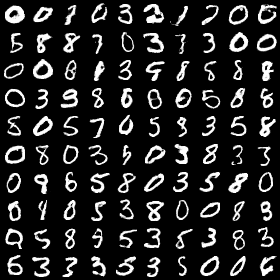
\includegraphics[width=0.8\textwidth]{img/gan_mnist_randomly_generated.png}
\caption{GAN}
\label{fig:gan_mnist_randomly_generated}
\end{subfigure}
\begin{subfigure}{.49\textwidth}
\centering
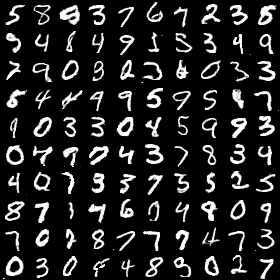
\includegraphics[width=0.8\textwidth]{img/capsgan_mnist_randomly_generated.png}
\caption{CapsuleGAN}
\label{fig:capsgan_mnist_randomly_generated}
\end{subfigure}
\label{fig:mnist_randomly_generated}
\caption{Randomly generated MNIST images}
\end{figure}

\begin{figure}
\centering
\begin{subfigure}{.49\textwidth}
\centering
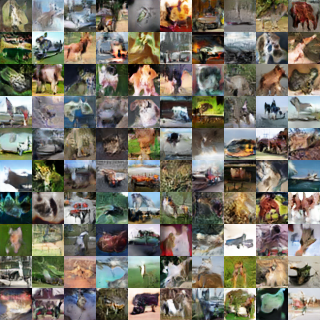
\includegraphics[width=0.8\textwidth]{img/gan_cifar10_randomly_generated.png}
\caption{GAN}
\label{fig:gan_cifar10_randomly_generated}
\end{subfigure}
\begin{subfigure}{.49\textwidth}
\centering
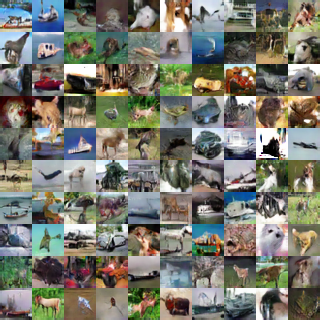
\includegraphics[width=0.8\textwidth]{img/capsgan_cifar10_randomly_generated.png}
\caption{CapsuleGAN}
\label{fig:capsgan_cifar10_randomly_generated}
\end{subfigure}
\label{fig:cifar10_randomly_generated}
\caption{Randomly generated CIFAR-10 images}
\end{figure}

\subsection{Visual Quality of Randomly Generated Images}

We qualitatively compare images generated randomly using both GAN and CapsuleGAN. Figures~\ref{fig:gan_mnist_randomly_generated}~and~\ref{fig:capsgan_mnist_randomly_generated} show images generated using the standard convolutional-GAN and CapsuleGAN, respectively, on the MNIST dataset. Qualitatively, both CapsuleGAN and the standard convolutional-GAN produce crisp images of similar quality, that sometimes do not resemble any digit. However, the image-grid generated using GAN seems to have less diversity in terms of generated classes of digits. Figures~\ref{fig:gan_cifar10_randomly_generated}~and~\ref{fig:capsgan_cifar10_randomly_generated} show the results of this experiment on the CIFAR-10 dataset. Both the models produce diverse sets of images but images generated using CapsuleGAN look cleaner and crisper than those generated using convolutional-GAN. We provide results of our quantitative evaluation in the following subsections for deeper analyses of the image generation performance.

\subsection{Generative Adversarial Metric}

Im et al.~\cite{bib:gam} introduced the generative adversarial metric (GAM) as a pairwise comparison metric between GAN models by pitting each generator against the opponent's discriminator, i.e., given two GAN models $M_1 = (G_1, D_1)$ and $M_2 = (G_2, D_2)$, $G_1$ engages in a battle against $D_2$ while $G_2$ against $D_1$. The ratios of their classification errors on real test dataset and on generated samples are then calculated as $r_{test}$ and $r_{samples}$. Following their implementation~\footnote{https://github.com/jiwoongim/GRAN/battle.py}, in practice, the ratios of classification accuracies are calculated instead of errors to avoid numerical problems, as shown in Equations \ref{eq:gam1} and \ref{eq:gam2}

\begin{equation}\label{eq:gam1}
r_{samples} = \frac{A(D_{GAN}(G_{CapsuleGAN}(\mathbf{z})))}{A(D_{CapsuleGAN}(G_{GAN}(\mathbf{z})))}
\end{equation}

\begin{equation}\label{eq:gam2}
r_{test} = \frac{A(D_{GAN}(\mathbf{x_{test}}))}{A(D_{CapsuleGAN}(\mathbf{x_{test}}))}
\end{equation}

Therefore, for CapsuleGAN to win against GAN, both $r_{samples} < 1$ and $r_{test} \simeq 1$ must be satisfied. In our experiments, we achieve $r_{samples} = 0.79$ and $r_{test} = 1$ on the MNIST dataset and $r_{samples} = 1.0$ and $r_{test} = 0.72$ on the CIFAR-10 dataset. Thus, on this metric, CapsuleGAN performs better than convolutional GAN on the MNIST dataset but the two models tie on the CIFAR-10 dataset.

\makegapedcells
\begin{table}
\centering
\caption{Results of semi-supervised classification - MNIST}
\label{tab:mnist_semi_supervised}
\begin{tabular}{ c ?{1.5pt} c | c | c }
  \hbline
  \textbf{Model} & \multicolumn{3}{c}{\textbf{Error Rate}} \\
  \hbline
  \nocell{1} & n = 100 & n = 1,000 & n = 10,000 \\ \cline{2-4}
  GAN & 0.2900 & 0.1539 & 0.0702 \\
  CapsuleGAN & \textbf{0.2724} & \textbf{0.1142} & \textbf{0.0531} \\
  \hbline
\end{tabular}
\end{table}

\makegapedcells
\begin{table}
\centering
\caption{Results of semi-supervised classification - CIFAR-10}
\label{tab:cifar10_semi_supervised}
\begin{tabular}{ c ?{1.5pt} c | c | c }
  \hbline
  \textbf{Model} & \multicolumn{3}{c}{\textbf{Error Rate}} \\
  \hbline
  \nocell{1} & n = 100 & n = 1,000 & n = 10,000 \\ \cline{2-4}
  GAN & 0.8305 & 0.7587 & 0.7209 \\
  CapsuleGAN & \textbf{0.7983} & \textbf{0.7496} & \textbf{0.7102} \\
  \hbline
\end{tabular}
\end{table}

\subsection{Semi-supervised Classification}

We evaluate the performance of the convolutional GAN and the proposed CapsuleGAN on semi-supervised classification. In this experiment, we randomly generate $50,000$ images using both GAN and CapsuleGAN. We use the Label Spreading algorithm~\cite{bib:label_spreading} with the generated images as the unlabeled examples and $n$ real labeled samples, with $n \in \{100, 1000, 10000\}$. We use the \texttt{scikit-learn}~\footnote{http://scikit-learn.org/} package for these experiments. Table~\ref{tab:mnist_semi_supervised} shows the results of our experiments on MNIST while Table~\ref{tab:cifar10_semi_supervised} shows those on CIFAR-10. The error rates are high in most experimental settings because we provide raw pixel values as features to the classification algorithm. However, this allows us to more objectively compare the two models without being biased by feature extraction methods. The results show that the proposed CapsuleGAN consistently outperforms convolutional GAN for all the tested values of $n$ with a margin of $1.7-3.97$ percentage points for MNIST and $0.91-3.22$ percentage points for CIFAR-10. Thus, CapsuleGAN generates images that are more similar to real images and more diverse than those generated using convolutional GAN, leading to better semi-supervised classification performance on the test dataset.

